\documentclass{article}
\usepackage[utf8]{inputenc}


\usepackage{tikz}
\usetikzlibrary{calc}

\begin{document}

\thispagestyle{empty}

\begin{figure}[h!]
		\centering
		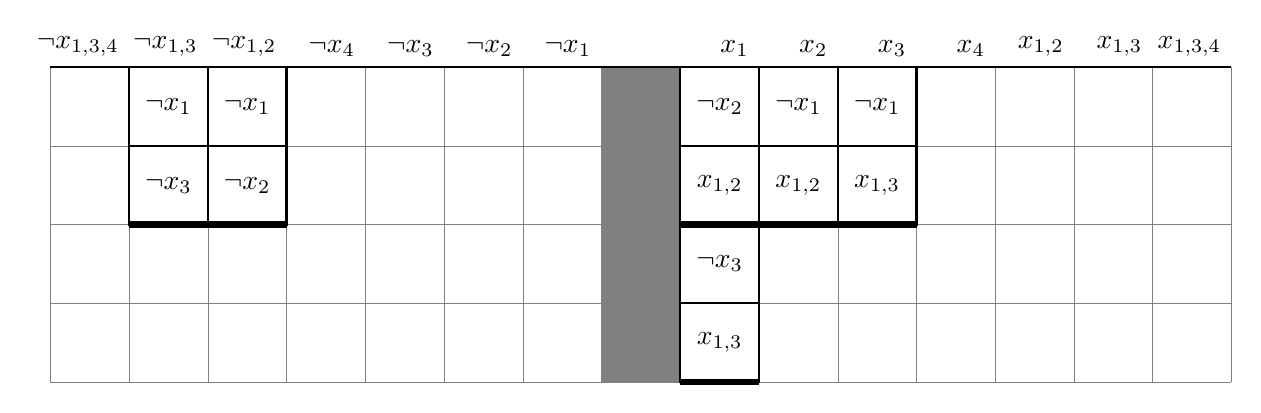
\begin{tikzpicture}
		%grid outline
		\draw[step=1cm,gray,very thin] (-7,0) grid (8,4);
		\fill[gray] (0,0) rectangle (1,4);
		
		%indexes
		\draw[thick] (-7,4) -- (-6,4) node[anchor=south east] {$\lnot x_{1,3,4}$};
		\draw[thick] (-6,4) -- (-5,4) node[anchor=south east] {$\lnot x_{1,3}$};
		\draw[thick] (-5,4) -- (-4,4) node[anchor=south east] {$\lnot x_{1,2}$};
		\draw[thick] (-4,4) -- (-3,4) node[anchor=south east] {$\lnot x_{4}$};
		\draw[thick] (-3,4) -- (-2,4) node[anchor=south east] {$\lnot x_{3}$};
		\draw[thick] (-2,4) -- (-1,4) node[anchor=south east] {$\lnot x_{2}$};
		\draw[thick] (-1,4) -- (0,4) node[anchor=south east] {$\lnot x_{1}$};
		\draw[thick] (0,4) -- (1,4);
		\draw[thick] (1,4) -- (2,4) node[anchor=south east] {$x_{1}$};
		\draw[thick] (2,4) -- (3,4) node[anchor=south east] {$x_{2}$};
		\draw[thick] (3,4) -- (4,4) node[anchor=south east] {$x_{3}$};
		\draw[thick] (4,4) -- (5,4) node[anchor=south east] {$x_{4}$};
		\draw[thick] (5,4) -- (6,4) node[anchor=south east] {$x_{1,2}$};
		\draw[thick] (6,4) -- (7,4) node[anchor=south east] {$x_{1,3}$};
		\draw[thick] (7,4) -- (8,4) node[anchor=south east] {$x_{1,3,4}$};
		
		%implications
		\draw[thick] (1,4) rectangle (2,3) node[pos=.5] {$ \lnot x_{2}$};
		\draw[thick] (1,3) rectangle (2,2) node[pos=.5] {$ x_{1,2}$};
		\draw[line width=0.8mm] (1,2) -- (2,2);
		
		\draw[thick] (1,2) rectangle (2,1) node[pos=.5] {$ \lnot x_{3}$};
		\draw[thick] (1,1) rectangle (2,0) node[pos=.5] {$ x_{1,3}$};
		\draw[line width=0.8mm] (1,0) -- (2,0);
		
		\draw[thick] (2,4) rectangle (3,3) node[pos=.5] {$ \lnot x_{1}$};
		\draw[thick] (2,3) rectangle (3,2) node[pos=.5] {$ x_{1,2}$};
		\draw[line width=0.8mm] (2,2) -- (3,2);
		
		\draw[thick] (-5,4) rectangle (-4,3) node[pos=.5] {$ \lnot x_{1}$};
		\draw[thick] (-5,3) rectangle (-4,2) node[pos=.5] {$ \lnot x_{2}$};
		\draw[line width=0.8mm] (-5,2) -- (-4,2);
		
		\draw[thick] (3,4) rectangle (4,3) node[pos=.5] {$ \lnot x_{1}$};
		\draw[thick] (3,3) rectangle (4,2) node[pos=.5] {$ x_{1,3}$};
		\draw[line width=0.8mm] (3,2) -- (4,2);
		
		\draw[thick] (-6,4) rectangle (-5,3) node[pos=.5] {$ \lnot x_{1}$};
		\draw[thick] (-6,3) rectangle (-5,2) node[pos=.5] {$ \lnot x_{3}$};
		\draw[line width=0.8mm] (-6,2) -- (-5,2);
		
		\end{tikzpicture}
		\caption{Lists of ternary implications. There is a delimiter between the tuples.}
		\label{fig:ternary_implications}
	\end{figure}

\end{document}
